\clearpage

\section{Setup}
\label{sec:setup}

In this section we explain how we set up the experiments with the cluster to see how it performs. We will later list these results and discuss and compare these to results from a MacBook Pro Late 2012.

\subsection{Introduction}
We plan on running these experiments in two phases, first to identify areas where improvement can be made along with bottlenecks and then after attempting to mitigate these to see if any improvement was made, and see where we end up.

We currently have 3 hardware configurations. The 8 node cluster can be split into:

\begin{enumerate}
\item 1 load distributor and 7 worker nodes
\item 8 worker nodes
\item 5 worker nodes (overclock)
\end{enumerate}

The overclock mode is reduced to 5 workers because the last 3 nodes refused to run properly at the overclocked speed.

In addition we will also look at the i5 MacBook with 1 and 2 threads.

\subsection{Setup}
The setup is the cluster of 8 PI-nodes. Since we are limited by the 8 ports on our switch, we have the load distributor and the load generator connected to another D-Link router that is then connected to the switch.
Also note that we need to be wary of this bottlenecking our total bandwidth to the 7 worker nodes through one cable.
This means we can at most hope to push 100Mbit/s of data to the workers {\em in total}.
The network layout is illustrated in Figure \ref{fig:network}.

\begin{figure}[h]
    \centering
    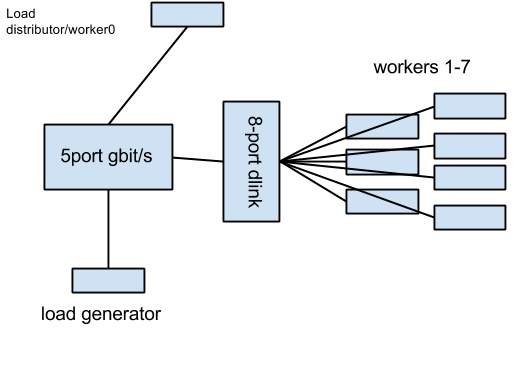
\includegraphics[width=0.8\textwidth]{experiments/networklayout}
    \caption{The network layout for the testing environment.}
    \label{fig:network}
\end{figure}


\subsection{Result gathering}
To obtain results we use a combination of controlling sending, output from the system and measuring the power consumed. To measure power usage we have a COITECH power consumption tool that is placed between the power outlet and our power adapters.
This lets us read the current power consumed by the whole system.

Our load generation utility has a few parameters for us to control. The number of queries to be sent, sending interval, number of threads and the set of nodes to which to send.

\subsection{MacBook Pro control}
When comparing on the MacBook, the load generator is run on a Mac Mini and the search program is run, either in one instance to test single core performance, or in two instances to utilize both the cores.
When running two instances these two operate on different ports.

\subsection{Overclocked Pis}
Overclocking is the process of making a computer operate at a faster clock rate than the manufacturer intended.
This is most often done by changing software parameters, typically by increasing the memory frequency, core frequency and/or operating voltage to make it stable at a higher clock rate.
Side effects of this process is an increase in power consumption and heat dissipation, and in some cases leads to system instability or even permanent damage to the components.

The Raspberry PI is very simple to overclock. By editing boot config-file one can easily change the CPU parameters.

This file can be found under:

\begin{lstlisting}
\boot\config.txt
\end{lstlisting}

\begin{lstlisting}
## Some overclocking settings, cpu govenor is set to ondemand

##None
#arm_freq=700
#core_freq=250
#sdram_freq=400
#over_voltage=0

##Modest
#arm_freq=800
#core_freq=300
#sdram_freq=400
#over_voltage=0

##High
#arm_freq=950
#core_freq=450
#sdram_freq=450
#over_voltage=6

##Turbo
arm_freq=1000
core_freq=500
sdram_freq=600
over_voltage=6
\end{lstlisting}

We went for the Turbo mode, which is the fastest recommended mode by the creators of Raspberry Pi that generally shows stable operation.
This mode increases the memory frequency by 50\%.  With {\tt core\_freq} set to 600, it doubles the GPU frequency which also drives the L2 cache for the CPU.
Doubling the L2 cache frequency is the main reason we chose Turbo mode, with synthetic tests showing over 50\% gains in performance\cite{overclock} from this overclock.
The L2 cache is really important as it is the main source of caching before the memory.

Unfortunately for us, only 5 of our units were able to run stable at the increased speed.
We saw both data corruption on the SD card, unable to completely boot, and general random runtime errors from three of the boards.
We therefore chose to do the overclocked tests with only 5 workers, seeing as the performance scales fairly linearly in our cases.
